\subsection{BWV2}

Os comandos \verb|python main.py -f 3| realiza a saída explicitada na \autoref{fig:bwv2_extract}. Novamente, é possível observar a mesma direcionalidade tessitural notada na \autoref{fig:bwv1_extract}.

\begin{figure}[h]
  \centering
  {%
\parindent 0pt
\noindent
\ifx\preLilyPondExample \undefined
\else
  \expandafter\preLilyPondExample
\fi
\def\lilypondbook{}%
\includegraphics{../examples/bwv2/bd/lily-90c88b91-1}%
\ifx\betweenLilyPondSystem \undefined
  \linebreak
\else
  \expandafter\betweenLilyPondSystem{1}%
\fi
\includegraphics{../examples/bwv2/bd/lily-90c88b91-2}%
\ifx\betweenLilyPondSystem \undefined
  \linebreak
\else
  \expandafter\betweenLilyPondSystem{2}%
\fi
\includegraphics{../examples/bwv2/bd/lily-90c88b91-3}%
% eof

\ifx\postLilyPondExample \undefined
\else
  \expandafter\postLilyPondExample
\fi
}

  \caption{Material musical gerado com o comando descrito anteriormente. \textbf{Fonte}: Autor.}
  \label{fig:bwv2_extract}
\end{figure}


Aplicando algumas intervenções,

\begin{figure}[!hb]
  \centering
{%
\parindent 0pt
\noindent
\ifx\preLilyPondExample \undefined
\else
  \expandafter\preLilyPondExample
\fi
\def\lilypondbook{}%
\includegraphics{../examples/bwv2/87/lily-e2caa734-1}%
\ifx\betweenLilyPondSystem \undefined
  \linebreak
\else
  \expandafter\betweenLilyPondSystem{1}%
\fi
\includegraphics{../examples/bwv2/87/lily-e2caa734-2}%
\ifx\betweenLilyPondSystem \undefined
  \linebreak
\else
  \expandafter\betweenLilyPondSystem{2}%
\fi
\includegraphics{../examples/bwv2/87/lily-e2caa734-3}%
\ifx\betweenLilyPondSystem \undefined
  \linebreak
\else
  \expandafter\betweenLilyPondSystem{3}%
\fi
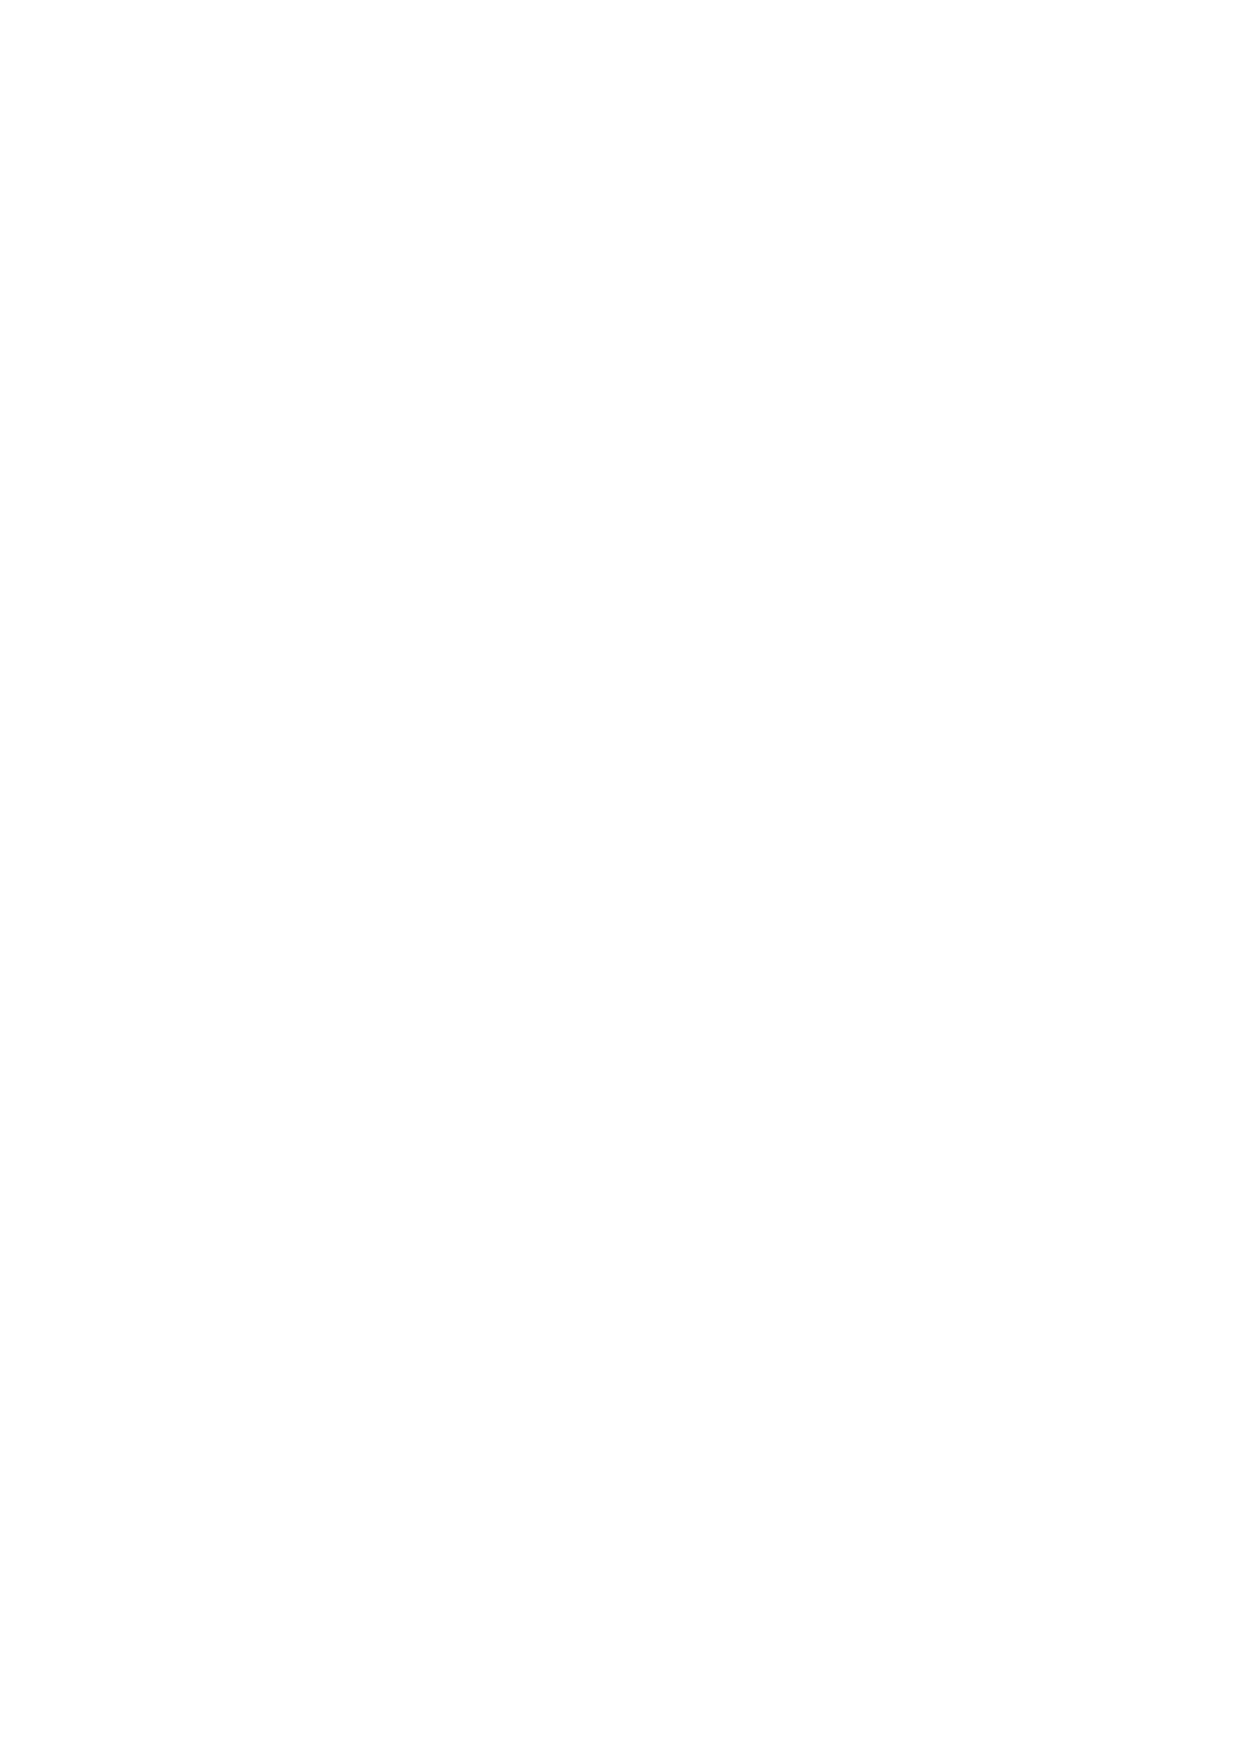
\includegraphics{../examples/bwv2/87/lily-e2caa734-4}%
% eof

\ifx\postLilyPondExample \undefined
\else
  \expandafter\postLilyPondExample
\fi
}

\caption{Peça final com aplicações das intervenções. \textbf{Fonte}: Autor.}
\label{fig:bwv2}
\end{figure}

